\documentclass[conference]{IEEEtran}
\usepackage[utf8]{inputenc}
\usepackage{ifpdf}
\renewcommand{\sfdefault}{cmss}
\renewcommand{\rmdefault}{cmr}
\renewcommand{\ttdefault}{cmtt}
\usepackage[english,russian]{babel}
\usepackage[pdftex]{graphicx}
\usepackage{caption}
\usepackage[colorlinks,filecolor=blue,citecolor=green,unicode,pdftex]{hyperref}
\usepackage{cmap}
\hypersetup{colorlinks=true, linkcolor=blue, citecolor=blue, filecolor=blue, urlcolor=blue, pdftitle=1, pdfauthor=, pdfsubject=, pdfkeywords=}

\begin{document}

\title{Тестирование среды программирования роботов}

\author{
	\IEEEauthorblockN{Д.А. Мордвинов}
	\IEEEauthorblockA{
		Санкт-Петербургский государственный университет\\
		Кафедра системного программирования\\
		Email: mordvinov.dmitry@gmail.com
	}
\and
	\IEEEauthorblockN{Ю.В. Литвинов}
	\IEEEauthorblockA{
		Санкт-Петербургский государственный университет\\
		Кафедра системного программирования\\
		Email: y.litvinov@spbu.ru
	}
}

\maketitle

\begin{abstract}
В статье представлен опыт тестирования достаточно сложной визуальной среды программирования роботов, 
написанной на C++ с использованием библиотеки Qt. Рассматриваются три аспекта тестирования среды --- 
модульное тестирование, тестирование пользовательского интерфейса и функциональное тестирование посредством 
интерпретации программ, написанных в среде, на имитационной модели с заданными ограничениями на состояние модели. 
Приводится описание языка задания ограничений. Описываются другие задачи, помимо тестирования, где представленные 
в статье решения оказались полезны --- код для тестирования пользовательского интерфейса переиспользован для 
реализации режима обучения, код для функционального тестирования переиспользован для проверки заданий учащихся 
онлайн-курса. Статья может быть полезна специалистом, занимающимся разработкой приложений на C++ с Qt и людям, 
занимающимся тестированием с использованием имитационных моделей физических объектов, которыми управляет программа.
\end{abstract}

\section{Введение}
C 2012 года ведётся разработка робототехнического конструктора ТРИК\footnote{Домашняя страница конструктора ТРИК, URL: http://www.trikset.com/ (дата обращения: 17.08.2015)} 
и графической среды программирования для него TRIK Studio~\cite{litvinov2015trikstudio}. Среда программирования 
появилась на базе наших исследований в области визуального моделирования (\cite{kuzenkova2013qreal, kuzenkova2011qreal, terekhov2009architecture}) 
и их приложения к робототехнике (\cite{terekhov2013robots, litvinov2012robots, tikhonova2012robots, bryksin2011robots}), 
так что на данный момент она представляет собой достаточно большую и богатую функциональными возможностями 
систему, имеющую несколько тысяч пользователей по всей стране и в мире. Среда предназначается прежде всего 
для обучения школьников и студентов программированию и робототехнике. Система имеет открытый исходный 
код, кроссплатформенная\footnote{Репозиторий проекта на GitHub, URL: http://github.com/qreal/qreal/ (дата обращения: 17.08.2015)} 
(на момент написания статьи работает под управлением операционных систем Windows, Linux и Mac OS X), реализована 
на языке C++ с использованием библиотеки Qt 5\footnote{Домашняя страница библиотеки Qt, URL: http://www.qt.io/ (дата обращения: 17.08.2015)}, 
содержит как развитый пользовательский интерфейс, так и сложную внутреннюю логику работы, включающую в 
себя управление реальными роботами и исполнение программ на имитационной модели. Это создаёт некоторые 
сложности в организации автоматического тестирования системы. В этой статье будет рассказано, как эти 
сложности преодолевались и как вообще было организовано автоматическое тестирование, что может быть полезно 
читателю как с чисто технической точки зрения (тестирование приложений с пользовательским интерфейсом, 
реализованных с использованием библиотеки Qt), так и с научной (тестирование среды программирования роботов 
посредством проверки корректности исполнения программ на имитационной модели).

Среда TRIK Studio представляет собой средство визуального программирования роботов, то есть среду, где 
программы представляются в виде набора графических символов (или блоков), реализующих элементарные команды 
роботу (включить моторы, дождаться срабатывания датчика и т.д.). Блоки соединены стрелками, показывающими 
передачу управления. Такой подход довольно типичен для данной предметной области (ближайшие аналоги TRIK Studio 
--- среды Robolab~\cite{portsmore1999robolab}, NXT-G\footnote{Среда программирования NXT-G, URL: http://www.lego.com/ru-ru/mindstorms/learn-to-program (дата обращения: 07.02.2015)}, 
MRDS\footnote{Microsoft Robotics Developer Studio, домашняя страница, URL: https://msdn.microsoft.com/en-us/library/bb648760.aspx (дата обращения: 07.02.2015)}). 
Одна и та же нарисованная программа может быть исполнена на компьютере с посылкой команд реальному роботу, сгенерирована в программу 
на JavaScript, F\# или C и передана роботу для исполнения в автономном режиме, или исполнена на имитационной 
модели, где симулируется робот и его окружение.

Автоматическое тестирование системы TRIK Studio состоит из трёх частей --- модульного тестирования, тестирования 
пользовательского интерфейса и функционального тестирования посредством имитационной модели. Первые две части 
типичны для практически любых приложений с пользовательским интерфейсом, третья же специфична для предметной 
области робототехники --- среда симулирует поведение реального робота и исполняет тестовые программы на нём, 
контролируя состояние среды симуляции посредством задания ограничений на её состояние, зависящих от времени и происходящих событий.

В статье будет рассказано про каждый из упомянутых выше этапов автоматического тестирования. Каждый этап 
представляет собой применение знаний из весьма обширной области, поэтому в данной работе не ставится цель подробно 
рассказать про модульное тестирование или тестирование пользовательского интерфейса вообще (это было бы слишком 
амбициозной задачей, к тому же уже решённой в многочисленных статьях и книгах, например, \cite{banerjee2013graphical, kotlyarov2006testing}). 
Цель данной работы --- представить опыт применения некоторых методик тестирования в реальном промышленном 
активно развивающемся проекте, представить и пояснить принятые нами решения.

\section{Модульное тестирование}
Для C++ существует множество библиотек модульного тестирования и единого стандарта не существует. Для выбора 
конкретной библиотеки мы руководствовались такими критериями, как скорость и простота написания теста, умение 
библиотеки работать с исключениями, наличие развитого механизма проверок, наличие поддержки создания mock-объектов. 

Библиотека Qt, на основе которой разрабатывается TRIK Studio, имеет в своём составе библиотеку модульного 
тестирования Qt Test\footnote{Документация по Qt Test, URL: http://doc.qt.io/qt-5/qttest-index.html (дата обращения 17.08.2015)}, 
но, несмотря на хорошую интеграцию с Qt, нам она не подошла по причине отсутствия встроенной поддержки работы с исключениями 
и mock-объектами. Также были рассмотрены библиотеки CPPUnit, Boost.Test, CppUnitLite, Unit++, CxxTest, Google C++ Testing Framework, 
подробное сравнение этих библиотек можно найти в работе~\cite{bazhutin2012course}. В результате была выбрана 
библиотека Google C++ Testing Framework\footnote{Домашняя страница Google C++ Testing Framework, URL: https://code.google.com/p/googletest/ (дата обращения: 07.02.2015)} 
и её расширение для написания mock-объектов Google C++ Mocking Framework\footnote{Домашняя страница Google C++ Mocking Framework, URL: https://code.google.com/p/googlemock/ (дата обращения: 07.02.2015)}.Эти инструменты удовлетворяют нашим критериям, кроме того, оказались просты в использовании, в том числе и в кроссплатформенном окружении. 

При написании тестов мы пытались поддерживать соответствие <<один исполняемый файл с тестами --- один бинарный файл системы 
(разделяемая библиотека или исполнимый файл)>>, структура тестов примерно повторяет структуру основного 
проекта. При этом возникла проблема, что операционная система Windows не позволяет передавать в командной 
строке слишком длинные пути (более 260 символов), поэтому пришлось несколько упростить в тестах иерархию 
каталогов, иначе возникали трудности со сборкой. Модульные тесты не раз доказали свою эффективность, помогая 
искать ошибки на ранних этапах разработки и упрощая рефакторинг.

\section{Тестирование пользовательского интерфейса}
Одно лишь модульное тестирование, по крайней мере в нашем случае, не может покрыть все аспекты системы. 
Пользовательский интерфейс также подлежит проверке корректности. Данный раздел содержит описание результатов 
поиска подходящего решения, подхода к тестированию пользовательского интерфейса в TRIK Studio, а также 
обсуждение некоторых прикладных сторон технологии, полученной в результате данного исследования.

\subsection{Существующие подходы}
Тестирование графических интерфейсов --- область, возраст которой составляет четверть века. За это время 
было опубликовано множество статей, проведена их подробная классификация (см.~\cite{banerjee2013graphical}), 
разработано большое количество подходов и инструментов, реализующих эти подходы. Данная работа не затрагивает 
фундаментальных теоретических оснований данной области, а скорее является практическим результатом на 
пересечении технологий, о которых будет рассказано в этом и последующих разделах.

TRIK Studio обладает сложным и постоянно изменяющимся интерфейсом, созданным на основе инструментария 
Qt Widgets\footnote{Документация по Qt Widgets, URL: http://doc.qt.io/qt-5/qtwidgets-index.html (дата обращения 17.08.2015)}. 
Кроссплатформенность системы предъявляет важное требование к технологии тестирования интерфейса --- одни 
и те же тесты должны иметь работать на различных операционных системах, оконных менеджерах, установленных 
разрешениях экрана и т.д. Открытость кода и свободное распространение среды делает непригодными коммерческие 
системы тестирования (например, Squish\footnote{Домашняя страница Squish, URL: http://www.froglogic.com/squish/gui-testing/ (дата обращения 17.08.2015)}, 
который пригоден по всем другим параметрам). Приведем обзор технологий, с которыми мы столкнулись в процессе 
поиска конечного решения задачи тестирования интерфейсов.

\subsubsection{Библиотека Qt Test}
Инструментарий Qt содержит набор средств автоматизации взаимодействия с пользовательским интерфейсом приложения, 
предоставляя библиотеку Qt Test в базовом некоммерческом модуле. Данный инструмент позволяет автоматизировать 
взаимодействие с графическим интерфейсом посредством задержек и эмулирования низкоуровневых событий мыши 
и клавиатуры. Высокоуровневые операции поиска и взаимодействия с определенными элементами управления, инструменты 
их поиска и определения отсутствуют в библиотеке Qt Test, тем не менее содержатся в том или ином виде в 
различных местах инструментария для создания самих интерфейсов. 

В результате тест с использованием данной библиотеки представляет собой модуль на C++, требующий самостоятельной 
реализации частых операций (например, создание операции drag-and-drop из одного места в другое с последующим 
использованием результатов этой операции), а также перекомпиляции тестов при изменении пользовательского 
интерфейса, что затрудняет их поддержку. Сами по себе эти факторы не кажутся слишком проблематичными, 
однако на практике показали себя довольно затрудняющими процесс создания и поддержки тестов, код получался громоздким.

Тем не менее, формально данная технология удовлетворяет всем нашим требованиям, тесты не зависят от платформы, 
изменение интерфейса требует сопоставимых изменений тестов.

\subsubsection{Windows Automation API}
Для тестирования пользовательского интерфейса Windows-приложений часто используются возможности операционной 
системы Windows, а именно Windows Automation API\footnote{Документация Windows Automation API на MSDN, 
URL: https://msdn.microsoft.com/en-us/library/windows/desktop/ff486375(v=vs.85).aspx (дата обращения 17.08.2015)}. 
Это набор функций, доступных как из .NET, так и для программ на C++, с помощью которых можно получить 
доступ к элементам пользовательского интерфейса, таким как кнопки, поля для ввода, списки и т.д., и симулировать 
события ввода. В составе Windows SDK\footnote{Домашняя страница Windows 10 SDK, URL: https://dev.windows.com/en-us/downloads/windows-10-sdk (дата обращения 17.08.2015)} 
поставляются программы Inspect и AccScope, использующие Automation API для того, чтобы показывать структуру 
и свойства элементов управления приложений. Существуют и полноценные библиотеки GUI-тестирования, такие как 
White\footnote{Страница проекта White на GitHub, URL: https://github.com/TestStack/White (дата обращения 17.08.2015)} 
или UI Automation Verify\footnote{Домашняя страница UI Automation Verify, URL: https://uiautomationverify.codeplex.com/ (дата обращения 17.08.2015)}, 
скрывающие от программиста сложность использования Automation API и позволяющие удобно писать тестовые 
сценарии на .NET, работая в терминах элементов пользовательского интерфейса.

Основной недостаток подобного подхода в нашем случае --- отсутствие кроссплатформенности и некоторая ориентированность 
на .NET (сам Automation API может использоваться и из кода на C++, но большинство библиотек к нему написаны на C\#), 
что хоть и не делает невозможным, но усложняет использование такого подхода.

\subsubsection{Sikuli}
Sikuli~\cite{yen2009sikuli} --- это свободный инструмент, разрабатываемый в MIT для скриптования пользовательских действий на 
основе изображений отдельных областей экрана. Тест представляет собой скрипт на языке Python, где в качестве 
примитива может быть использовано изображение какого-либо фрагмента экрана. Инструмент предоставляет удобную 
среду программирования таких скриптов Sikuli IDE, которая позволяет быстро создавать и менять изображения прямо в коде теста.

Удобство написания простых тестов намного выше, чем при использовании библиотеки Qt Test, а также исчезает 
ряд проблем взаимодействия с операционной системой, однако данный инструмент не подошел нам из-за требований 
кроссплатформенности тестов. Очевидно, что на различных платформах и даже в разных версиях одной и той же 
платформы интерфейс приложения может выглядеть совершенно по-разному. При незначительной модификации интерфейса 
зачастую приходилось полностью изменять содержимое тестов. В итоге, несмотря на удобство и легкость написания 
простых тестов, данное обстоятельство делает Sikuli непригодным в нашем случае.

\subsection{Скриптовый программный интерфейс}
\label{part:scriptApi}
В результате так и не было найдено готового решения, способного удовлетворить всем поставленным ограничениям. 
Наиболее близкой к желаемому оказалась библиотека Qt Test, которая представляет собой скорее основу для
технологии тестирования интерфейсов, чем саму технологию. Опыт использования описанных решений позволил 
нам сформировать представление о платформе, обладающей всеми достоинствами Qt Test в виде кроссплатформенности 
и возможности создания самой изощренной логики тестирования и простотой и лаконичностью скриптового подхода наподобие Sikuli.

В нашем представлении подходу с использованием Qt Test не хватает <<скриптовости>> и высокоуровневости 
в смысле работы в терминах элементов управления, а не событий от манипуляторов. Эти идеи были учтены при 
реализации системы тестирования интерфейсов TRIK Studio.

В качестве основного языка написания тестов был выбран Qt Script. Это реализация стандарта 
ECMAScript\footnote{Домашняя страница ECMAScript, URL: http://www.ecmascript.org/ (дата обращения 17.08.2015)} 
(наиболее популярной реализацией которого является язык JavaScript), расширенная механизмами интеграции 
с Qt-приложениями. Скриптовое окружение расширено инструментами работы с пользовательским интерфейсом системы 
в терминах самого интерфейса. Работа этого окружения осуществляется посредством библиотек Qt Test и Qt Widgets, 
таким образом, сохраняются независимость тестов от платформы и легкость доступа ко всем элементам управления, 
при этом решаются проблемы громоздкости кода тестов и низкоуровневости терминов, в которых они работают.

Окружение предоставляет доступ ко всем частям интерфейса и методам работы с ними и содержит вспомогательную функциональность, 
специфичную только для TRIK Studio. К примеру, существует возможность скриптования создания визуальных диаграмм, 
рисования модели мира, в котором будет производиться имитационное моделирование робота, работы с жестами мышью, 
изменения свойств примитивов, из которых строится программа, работы с настройками приложения, управления 
состоянием вспомогательных панелей и т.д. Реализованы также методы произвольного доступа к элементам управления 
интерфейса по структурному описанию (идентификаторам и/или положению в дереве элементов управления) и координатам 
на экране. Управление эмуляторами устройств ввода (например, навигация и действия виртуальной мышью или указание 
клавиатурного фокуса и последовательностей нажатий на кнопки клавиатуры) тесно интегрировано с различными 
видами элементов управления. Например, присутствуют отдельные функции прокрутки и работы с выпадающими 
списками. При этом остаются доступными методы синтезирования низкоуровневых событий манипуляторов. 

Кроме всего описанного, скриптовый интерфейс системы содержит методы показа информационных сообщений, подсвечивания 
отдельных элементов управления и рисования стрелок-указателей на них, анимации виртуального курсора мыши 
и тому подобных <<показательных>> функций, надобность которых будет обсуждаться в разделе~\ref{part:demos}. 
Тем не менее, остаются открытыми некоторые проблемы, каждая из которых носит чисто технический характер. 
Одна из них --- управление системными диалоговыми окнами. Дело в том, что на каждой платформе системные 
диалоговые окна (такие как диалоги выбора файлов, печати, выбора цвета и т.д.) свои и не поддаются контролю 
системы синтезирования событий, используемой в библиотеке Qt Test. Сейчас эта проблема обходится работой 
с этими диалогами как с <<черными ящиками>> --- тесты задают для себя результаты выбора сущностей, редактируемых 
этими диалогами, не прибегая к работе с ними, <<обходя>>, таким образом, их на уровень выше. Другая проблема 
--- отсутствие в Qt Test возможности эмулирования ввода с клавиатуры на разных языках, что делает невозможным 
полноценное тестирование локализации среды. Все эти проблемы являются, скорее, проблемами библиотеки Qt Test, 
в то время как с нашей стороны единственной на данный момент проблемой является стоимость поддержки кодовой базы, 
что, безусловно, являясь значимым, не будет обсуждаться в рамках этой статьи.

Полученная технология оказалась практически полностью удовлетворяющей нашим потребностям в удобстве написания 
тестов и их переносимости. Важно, что разработкой автоматизированного тестирования интерфейса смогли заниматься 
люди, практически не имеющие отношения к разработке и поддержке самой системы и не имеющие опыта программирования на C++.

\subsection{Инфраструктура}
В данном разделе будет кратко описана структура технологии тестирования, описанной в разделе~\ref{part:scriptApi}. 
Общая архитектура всего комплекса представлена на рисунке~\ref{image:architecture}. Основная идея состоит 
в создании новой <<прослойки>> системы, стоящей над всей технологией, интерфейса программирования поведения 
пользовательского интерфейса. Этот уровень не модифицирует кодовую базу системы, тем не менее агрегируя в 
себе все ее отдельные компоненты. Здесь реализуются все операции, специфичные только для данной платформы 
в удобном для использования в скриптах виде, а также происходит <<оборачивание>> операций библиотеки Qt Test. 
Интерпретатор Qt Script, занимающийся исполнением кода самих тестов, импортирует символы скриптового API. 
Очевидно, что необходимости в Qt Script в такой архитектуре нет, можно создавать тесты и на компилируемых 
языках, компонуясь с интерфейсом программирования, в этом случае такой новый уровень можно рассматривать 
просто как инструмент повторного использования кода в тестах.

\begin{figure}[!t]
	\centering
	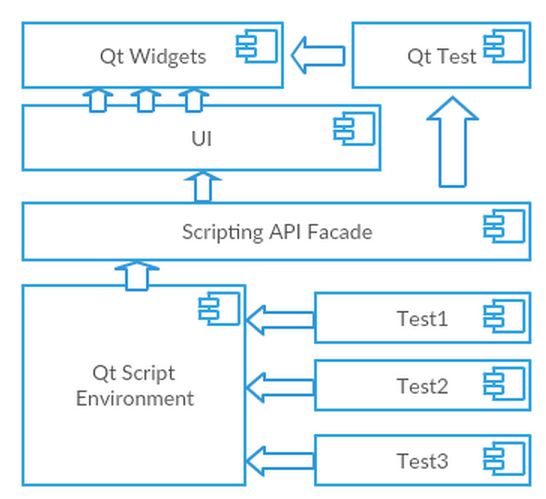
\includegraphics[width=2.5in]{guiTestingArchitecture.png}
	\caption{Архитектура системы тестирования интерфейсов TRIK Studio.}
	\label{image:architecture}
\end{figure}

\subsection{Использование технологии для обучения пользователей}
\label{part:demos}
Полученная технология обладает одним интересным приложением. На базе одной и той же инфраструктуры могут 
быть получены как тесты пользовательского интерфейса, так и автоматизированные демонстрации процесса работы 
со средой, встроенные прямо в нее. Это способ обучения пользователя возможностям среды, используемый, в 
основном, в компьютерных играх --- про возможности продукта рассказывает сам продукт (в противоположность, 
например, таким подходам как текстовая справка или видео уроки).

Возможно, такой подход будет полезен разработчикам приложений с развитым, нестандартным графическим интерфейсом. 
Написанием скриптов тестирования и скриптов демонстрации могут заниматься одни и те же люди, даже не участвующие 
в написании кода самого приложения.

\subsection{Обсуждение}
Дальнейшее развитие этой технологии предполагает генерацию скриптов симуляции поведения пользователей. В самом 
простом случае тесты графического интерфейса и встроенные демонстрации возможностей среды можно создавать, 
записывая действия пользователя, работающего со средой. Если же требуется более сложная логика работы сценария, 
её можно описать с помощью специального визуального языка, по которому будет автоматически сгенерирован код 
скрипта тестирования. На данный момент эти технологии реализованы в системе TRIK Studio и проходят апробацию, 
но в силу того, что окончательный результат ещё не получен, они не будут подробно обсуждаться в рамках данной работы.

Разумеется, создание специального визуального языка для нужд тестирования пользовательского интерфейса <<с нуля>> 
было бы неоправданно трудозатратно. Однако такой подход полностью соответствует парадигме предметно-ориентированного 
моделирования (Domain-Specific Modeling~\cite{mernik2005and}), а визуальный язык и инструментальные средства 
к нему можно быстро реализовать с помощью так называемых DSM-платформ (\cite{pavlinov2006dsmtools, kelly2008domain}). 
Проект, на котором основывается TRIK Studio, QReal --- это пример такой DSM-платформы (на самом деле, 
сам язык программирования роботов и редактор к нему были созданы с помощью QReal в течение нескольких часов). 
Создать ещё один визуальный язык для тестирования пользовательского интерфейса TRIK Studio не представляло особой сложности.

Идея записи пользовательских действий с последующей генерацией теста уже находила свою реализацию, например, 
в проекте TPTP\footnote{Страница TPTP GUI Recorder, URL: http://www.eclipse.org/tptp/test/documents/userguides/Intro-Auto-GUI.html (дата обращения 17.08.2015)} 
тестирования приложений, созданных в среде разработке Eclipse\footnote{Домашняя страница проекта Eclipse, URL: https://eclipse.org/ (дата обращения 17.08.2015)}. 
Более того, существуют работы, в которых эта методика расширяется добавлением элементов искусственного 
интеллекта, например~\cite{memon2001hierarchical, sugiura1996simplifying}. Интеграция подобных подходов в наше решение 
является интересной темой дальнейших исследований.

\section{Функциональное тестирование}
\subsection{Краткое описание возможностей среды}
Далее в этом разделе пойдёт речь о тестировании функциональности, специфичной для TRIK Studio (и аналогичных 
систем, предназначенных для управления некоторым объектом), поэтому следует описать подробнее функциональность, 
которую требуется тестировать. 

TRIK Studio представляет собой среду программирования роботов на визуальном языке. Система поддерживает программирование 
робототехнических конструкторов Lego Mindstorms NXT 2.0, Lego Mindstorms EV3 и ТРИК, в разработке находится 
поддержка платформы Arduino. Для каждой из поддерживаемых платформ имеется возможность отладки визуальной 
программы на компьютере с посылкой команд роботу, генерации кода на каком-либо текстовом языке программирования 
(например, C, JavaScript, F\#, ШАЯ) с последующей загрузкой кода на робота по различным интерфейсам (Bluetooth, 
USB, Wi-Fi) для автономного исполнения. Существует также возможность отладки программы на двумерном виртуальном исполнителе.
Общий вид интерфейса среды представлен на рисунке~\ref{image:trikStudio}

\begin{figure*}[!t]
	\centering
	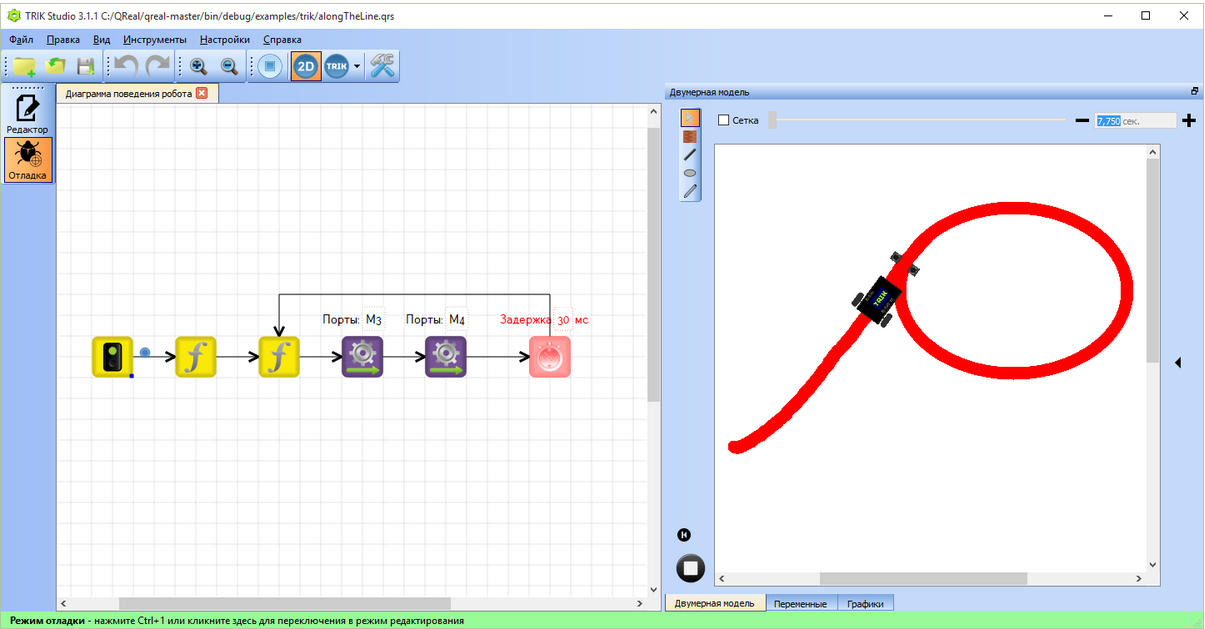
\includegraphics[width=7in]{trikStudio.png}
	\caption{Интерфейс TRIK Studio.}
	\label{image:trikStudio}
\end{figure*}

Программа представляется в виде набора блоков, каждый из которых представляет собой элементарную команду 
роботу или элементарный шаг вычисления. Команды роботу могут быть как простыми (например, включить мотор 
на таком-то порту с такой-то мощностью), так и довольно сложными (например, получить данные датчика линии, 
использующего видеокамеру и алгоритмы распознавания изображений), сложные алгоритмы, как правило, реализуются 
на самом роботе и среда лишь вызывает их и обрабатывает результаты. Во всех блоках можно использовать математические 
выражения на текстовом языке, представляющем собой подмножество языка Lua 5.3\footnote{Домашняя страница языка Lua, URL: http://www.lua.org/ (дата обращения 17.08.2015)}, 
синтаксический анализатор и интерпретатор которого были специально реализованы в TRIK Studio (готовые решения нас 
не устраивали тем, что невозможно было использовать их абстрактное синтаксическое дерево для генерации кода 
на других языках программирования, кроме того, над Lua пришлось реализовать свою систему типов, потому что 
некоторые целевые языки генерации, такие как C, статически типизированы). В выражениях можно использовать 
текущие значения датчиков робота, доступные как специальные переменные, они же отображаются в виде таблицы 
или графиков при запущенной в режиме интерпретации программе. В режиме генерации и автономного исполнения 
обращения к таким переменным транслируются в команды чтения значений датчиков и их показания на компьютере 
не отображаются (чтобы дать возможность программе исполняться автономно).

Двумерная модель позволяет исполнять большую часть программ, которые могут быть исполнены на реальном роботе. 
Пользователь может нарисовать в области редактирования двумерной модели стены, цветные линии или области на полу, 
разместить самого робота и его датчики, задать им направление. Датчики будут взаимодействовать со стенами и 
цветными линиями (для ТРИК поддержаны инфракрасные и ультразвуковые датчики расстояния, датчик освещённости и 
детектор линии по видеокамере, для Lego NXT или Lego EV3 --- все датчики, входящие в стандартный набор: касания, 
света, цвета и ультразвуковой датчик расстояния). Часть функциональности, доступная только на реальном роботе, 
имитационной моделью не поддерживается, например, на данный момент на имитационной модели может быть только один 
робот, поэтому в поддержке функциональности общения между роботами нет смысла. Тем не менее, имитационная модель 
позволяет решать большинство задач из курсов по робототехнике для Lego NXT (например,~\cite{filippov2013robotics}) 
и ТРИК\footnote{например, набор уроков И.Ю. Широколобова, URL: http://bit.ly/TRIK\_presentations (дата обращения 17.08.2015)}, 
и существенно упрощает отладку, давая возможность отладить алгоритм без реального робота, а потом лишь 
подобрать коэффициенты для исполнения той же программы в реальном мире.

Отдельно стоит отметить наличие достаточно развитых средств обеспечения удобства пользовательского интерфейса, 
что связано с образовательной направленностью среды. Например, при рисовании диаграмм можно пользоваться механизмом 
распознавания жестов мышью (\cite{osechkina2012multistroke}) --- с зажатой правой кнопкой рисуется схематичная фигура, которая распознаётся средой 
и на месте нарисованной фигуры создаётся соответствующий ей блок, что позволяет не искать нужный блок в палитре 
и сделать использование среды интереснее для детей. Для TRIK Studio проводились исследования по юзабилити 
и вносились правки в интерфейс по их результатам (\cite{sokovikova2012usability, kuzenkova2013course}).

Генерация кода для автономного исполнения на данный момент реализована для Lego NXT в язык C (с использованием 
библиотеки ECRobot\footnote{Домашняя страница ECRobot, URL: http://lejos-osek.sourceforge.net/html/index.html (дата обращения 17.08.2015)} 
и ОСРВ nxtOSEK\footnote{Домашняя страница nxtOSEK, URL: http://lejos-osek.sourceforge.net/ (дата обращения 17.08.2015)}) 
и для ТРИК в языки JavaScript (\cite{terekhov2013qreal}) и F\# (\cite{kirsanov2014robotics}). Для ТРИК 
также реализованы библиотеки поддержки времени выполнения на C++ и F\#, которые работают непосредственно 
на роботе и, собственно, реализуют функции, вызываемые программами, сгенерированными в TRIK Studio.

\subsection{Общая схема функционального тестирования}

Поскольку имитационная модель покрывает достаточно большой процент функциональности среды и ввиду сложности 
использования реального робота в автоматических тестах, именно имитационная модель используется нами для 
функционального тестирования. Обычно в аналогичных ситуациях пишется эмулятор реального устройства, у нас же 
эмулятор фактически является неотъемлемой частью системы и активно используется конечными пользователями. 
Предлагаемый подход к функциональному тестированию TRIK Studio таков:

\begin{enumerate}
	\item На визуальном языке рисуется программа для исполнения на имитационной модели, решающая ту или 
			иную практическую задачу, а также рисуется модель мира для имитационной модели, с которым эта программа будет работать.
	\item Программа снабжается описанием ограничений на состояние системы на специальном XML-языке, описание 
			которого приводится ниже. Наборов ограничений для одной программы может быть несколько, при этом 
			они могут использовать разные модели мира.
	\item Файл с сохранённой программой запускается на интерпретацию в двумерной модели, для этого используется 
			специально созданный для нужд тестирования исполняемый файл, представляющий собой по сути TRIK Studio 
			без пользовательского интерфейса. Тестирующая программа перед запуском тестируемой программы подменяет 
			модель мира и набор ограничений в сохранении, что даёт возможность использовать несколько тестов 
			для одной программы. Программа исполняется так, как она исполнялась бы, будучи запущенной пользователем 
			в TRIK Studio, и в случае, если одно из ограничений не выполнено, программа работает некорректно --- делается 
			вывод, что поведение интерпретатора или среды имитационного моделирования отличается от эталонного, 
			тест не пройден.
	\item Тестирующая программа вызывается системой непрерывной интеграции Travis\footnote{Система непрерывной интеграции Travis, URL: https://travis-ci.org/ (дата обращения 17.08.2015)} 
			каждый раз после сборки проекта, для всех файлов сохранений и моделей мира для них, имеющихся в репозитории.
	\item Результаты тестов рассылаются по электронной почте разработчикам.
\end{enumerate}

Архитектурно тестирующая система представляет собой отдельную программу, использующую в качестве
разделяемых библиотек ядро и имитационную модель системы TRIK Studio. При этом она
активно использует рефлексию, реализованную для C++ в библиотеке Qt для доступа к свойствам
объектов имитационной модели. Таким образом, при расширении возможностей системы или добавлении
нового вида симулированного оборудования новые объекты и свойства будут немедленно доступны из 
описаний ограничений, без дополнительной модификации кода. Тестовая система подписывается 
на события имитационной модели и вызывает проверку ограничений на каждом <<тике>> 
модельного времени. При этом проверяются только активные ограничения, которых в каждый 
конкретный момент времени немного, поэтому скорость работы оказывается вполне удовлетворительной.

\subsection{Описание языка задания ограничений}
Описание ограничений на имитационную модель робота производится на событийном языке, основанном на XML, разработанном 
как дополнение к механизму имитационного моделирования в среде. Выбор в пользу XML-фронтэнда был произведен 
из чисто практических соображений удобства интеграции с описанием остальной имитационной модели.

Программа на таком языке представляет собой множество $\{ e_1, e_2, ..., e_n \}$ событий, где каждое событие 
$e_i$ --- это тройка $(id_i, c_i, T_i)$.

\begin{itemize}
	\item $id_i$ --- идентификатор события, внутренняя метка, по которой к событию $e_i$ смогут обращаться другие события.
	\item $c_i$ --- условие срабатывания события, формула логики первого порядка, о предикатных и функциональных символах которой будет рассказано чуть ниже.
	\item $T_i$ --- упорядоченный список элементарных триггеров $[ t_{i1}, t_{i2}, ..., t_{in} ]$. Элементарный триггер --- это некоторое 
			действие, выполняемое в момент истинности условия срабатывания события $c_i$.
\end{itemize}

Одному событию соответствует один элемент в XML-спецификации программы. Каждое событие в текстовом описании 
программы может быть представлено либо в виде ограничения, либо в каноническом виде.

Событие в канонической форме --- уже описанная тройка $(id_i, c_i, T_i)$.

Событие в форме ограничения --- это событие вида $(id_i, !c_i, [ fail(message_j) ])$, где <<!>> означает 
логическое отрицание, а $fail(message_j)$ --- триггер прекращения исполнения имитационной модели с выдачей 
сообщения об ошибке $message_j$. Другими словами, ограничение --- это событие, которое срабатывает тогда, 
когда нарушается какое-то условие, и которое сообщает об этом нарушении. Особый случай такого ограничения --- 
лимит времени на выполнение программы. Такое ограничение должно присутствовать в любой программе проверки 
ограничений имитационной модели TRIK Studio (что проверяется на уровне самого языка задания ограничений), 
так как проверка, очевидно, не может осуществляться бесконечное время. 

Хоть в выделении ограничений в отдельную группу событий особой надобности нет, на практике удобно описывать 
утверждения вида <<робот x не должен выезжать за пределы зоны z>> или <<к роботу x должен быть подключен набор датчиков s>>
именно в терминах ограничений, а не событий.

Коротко опишем множество доступных в языке предикатных и функциональных символов и элементарных триггеров. 
Предикатные символы можно поделить на несколько групп:
\begin{itemize}
	\item Предикаты сравнения значений функциональных символов $>$, $<$, $<=$, $>=$, $=$, $!=$.
	\item Пространственные предикаты. Имеют вид <<тело x находится внутри области y>>.
	\item Предикаты состояния событий $settedUp(id_i)$ и $dropped(id_i)$, описывающие состояние события 
			(взведено/опущено). Во взведенном состоянии событие может быть выполнено, в опущенном оно 
			остается неактивным, не выполняя триггеры даже при выполнении условия срабатывания события.
	\item Предикат времени $timer(t)$, истинный в моменты времени $t$ и позже.
	\item Прочие предикаты, являющиеся надстройками над уже описанными и поддержанные в целях удобства.
\end{itemize}

Функциональные символы бывают следующих видов:
\begin{itemize}
	\item Константы различных типов (целочисленные, с плавающей точкой, строковые, логические, цветовые, геометрические и пр.).
	\item Символ $variableValue(id)$ для получения значения переменной с идентификатором $id$. Переменные 
			могут быть полезны при сложной логике проверки, например, при подсчете числа проделанных роботом итераций.
	\item Арифметические и геометрические операции над значениями других символов, например, модуль числа, 
			подсчет расстояния между двумя точками или выпуклая оболочка множества точек.
	\item Символы сравнения формы двух объектов с использованием расстояния Левенштейна, полезные при 
			проверке схожести фигур, нарисованных роботом.
	\item Символ $objectState(path)$ --- основное средство получения информации о состоянии устройств 
			робота и свойствах предмета из внешнего мира. Аргумент $path$ --- путь к желаемому свойству 
			в иерархии объектов в модели мира. Подробный рассказ обо всех свойствах, предоставляемых окружением, 
			довольно громоздкий и выходит за рамки данной статьи.
\end{itemize}

Наконец, элементарные триггеры делятся на следующие категории:
\begin{itemize}
	\item $success$, $fail(message)$ --- управление состоянием проверки. Первый помечает результат проверки 
			как успешный, второй --- как неудавшийся, отображая заданное сообщение об ошибке.
	\item Триггеры задания значения переменных и изменения значения свойств объектов из имитационной модели мира.
	\item Триггеры управления состоянием событий. Каждое событие может взвести или опустить другое или себя, 
			с помощью этого механизма можно задавать сложную логику проверки.
\end{itemize}

Пример простейшей программы на языке задания ограничений имитационной модели мира в TRIK Studio приведён в листинге~\ref{code:constraints}.

\captionsetup[figure]{name=Листинг}
\setcounter{figure}{0}

\begin{figure*}[!t]
\begin{verbatim}
<!-- Корневой элемент, означающий начало программы проверки ограничений -->
<constraints>

    <!-- Обязательное в любой программе ограничение на время работы -->
    <timelimit value="2000"/>

    <!-- Ограничение на местоположение робота -->
    <constraint failMessage="Робот покинул допустимую зону!">
        <inside objectId="robot1" regionId="warzone"/>
    </constraint>

    <!-- Условие успешности программы: робот должен сказать "Привет" с помощью
        встроенного механизма синтезирования речи и нарисовать улыбку на дисплее -->
    <event settedUpInitially="true">
        <conditions glue="and">
            <equals>
                <objectState object="robot1.shell.lastPhrase"/>
                <string value="Привет"/>
            </equals>
            <equals>
                <objectState object="robot1.display.smiles"/>
                <bool value="true"/>
            </equals>
        </conditions>
        <trigger>
            <success/>
        </trigger>
    </event>

</constraints>
\end{verbatim}
\caption{Пример программы проверки ограничений имитационной модели мира в TRIK Studio.}
\label{code:constraints}
\end{figure*}

\subsection{Использование для проверки заданий в онлайн-курсе}
Та же система, что используется для тестирования среды, используется и для проверки задач, решаемых пользователями 
в рамках онлайн-курса по робототехнике, подготавливаемого в данный момент для платформы Stepic\footnote{Платформа онлайн-обучения Stepic, URL: https://stepic.org/ (дата обращения 17.08.2015)}.
На сервере размещён набор задач в виде файлов сохранения TRIK Studio, в которых готова (и закрыта для модификации) модель 
мира для имитационной модели, некий набор ограничений, но не до конца нарисована программа (или отсутствует вовсе). 
Учащимся предлагается скачать файл с сохранением, открыть его в TRIK Studio, дорисовать программу, проверить, 
что программа работает у них в имитационной модели и удовлетворяет ограничениям, записанным в файле сохранения, 
и загрузить программу на сервер.

На сервере используется та же программа тестирования, которая подменяет модель мира и набор ограничений на тестовые
и запускает на исполнение пользовательскую программу. Возможность подменить модель мира позволяет проверить 
программу на работоспособность в различных (возможно, не известных пользователю заранее) условиях, а различные 
ограничения позволяют управлять случайными факторами, влияющими на работу программы (например, датчиком 
случайных чисел, или симулировать ввод пользователя). По результатам пользователю отправляется сообщение с результатом проверки.

Результат работы программы может быть отображён в браузере пользователя с помощью JavaScript-программы, рисующей 
двумерную модель и поведение робота в ходе выполнения задачи. Для этого сервер также готовит и отправляет по 
запросу файл с трассой робота --- набором пройденных им точек и состоянием подключенных к нему устройств. 
Некоторые задачи могут быть решены прямо в браузере, без открытия сохранения в TRIK Studio, для этого используется 
среда программирования, частично реализующая возможности TRIK Studio на JavaScript. Среда позволяет нарисовать 
диаграмму, после чего формирует файл сохранения TRIK Studio, который открывается системой проверки.

\subsection{Результаты}
На данный момент с помощью предлагаемой технологии реализовано 20 тестовых задач и
тестовая утилита, запускающая все задачи и контролирующая корректность работы системы.
Эти же тестовые задачи используются как упражнения для онлайн-курса%
\footnote{пример такой задачи доступен по ссылке http://bit.ly/online\_task\_demo (дата обращения: 01.11.2015)}
и покрывают функциональность от самой простой (проехать вперёд) до довольно сложной
(движение по лабиринту с использованием ультразвукового датчика расстояния). Все блоки,
доступные пользователю, встречаются хотя бы один раз в наборе тестов, кроме того, тесты фактически 
строятся по материалам годового курса обучения школьников, что даёт уверенность в
удовлетворительном покрытии типичных случаев использования имитационной модели. Прогон
полного набора существующих на данный момент тестов занимает порядка минуты, что позволяет запускать
тесты после каждого коммита в систему контроля версий.

На создание задач, ограничений на XML-языке и эталонных решений, которые, собственно,
и используются для тестирования среды, ушло примерно две человеконедели. В результате
тестирования было выявлено и исправлено порядка 10 дефектов имитационной модели, в том числе
и редко проявляющиеся при <<обычном>> использовании проблемы с зависимостью показаний,
возвращаемых некоторыми датчиками, от случайных факторов. Таким образом, технология 
уже оказалась нам полезна.

\section{Заключение}
В статье было рассмотрено применение ряда методик тестирования в проекте TRIK Studio. Было показано, что 
некоторые технологии полезны не только для тестирования, но и для реализации пользовательской функциональности: 
средство для тестирования пользовательских интерфейсов переиспользовано для реализации режима обучения пользователей, а 
средство для тестирования работы интерпретатора программ и имитационной модели --- для проверки заданий учащихся в онлайн-курсе.

Подходы, рассматриваемые в этой работе допускают интересные, на наш взгляд, обобщения и углубленное исследования.
В частности, интересными представляются идеи использования формальной верификации по методу Model Checking в 
функциональном тестировании среды программирования. Данное направление исследований интересно еще и потому, что на момент 
написания статьи находится в разработке событийный визуальный язык для программирования сложных мультиагентных 
систем, где результаты такого исследования, как представляется, могут быть эффективно применены.

\bibliographystyle{utf8gost705u}
\bibliography{bibliography}

\end{document}